\chapter{Anforderungen}
\label{ch:requirements}
In diesem Kapitel werden die Anforderungen für den im vorherigen Kapitel aufgezeigten Anwendungsfall aufgestellt. Ziel ist es, die \ac{DLT}-relevanten Anforderungen zu identifizieren, um dadurch im nächsten Kapitel eine geeignete \ac{DLT}-Lösung zu finden. Dazu werden zunächst einige Standards vorgestellt, wie Anforderungen klassifiziert und eingeordnet werden können. Diese Standards werden anschließend in einem optimierten Modell zusammengeführt und auf die konkreten Anforderungen angewandt. Die Klassifizierung dient als Werkzeug zur Einteilung der unübersichtlichen Gesamtmenge der Anforderungen und soll die weitere Identifikation \ac{DLT}-relevanter Anforderungen vereinfachen. Als Zwischenergebnis existieren verschiedene Anforderungsklassen, die auf \ac{DLT}-Relevanz geprüft werden. Durch schrittweises Ausschließen und Reduzieren der Anforderungsklassen werden jene Klassen identifiziert, die für die Umsetzung auf einer \ac{DLT}-basierten Lösung entscheidend sind.

%
% Section: Standards und Normen
%
\section{Standards und Normen}
\label{sec:requirements:standards}
In diesem Abschnitt werden die verwendeten Standards und Normen aufgelistet und kurz beschrieben:
\begin{description}
  \item[BABOK] Das \ac{BABOK} wird vom \ac{IIBA} herausgegeben und stellt einen Leitfaden für die Business-Analyse dar, genauere Informationen können \cite{BABOK} entnommen werden. Es unterteilt in sogenannte Knowledge-Areas und vermittelt Techniken und Kompetenzen im Umfeld der Business-Analyse. Anforderungen werden im \ac{BABOK} nach Abstraktionsebene gruppiert: Die Business-Ebene, die Anforderungen abstrakt aus Sicht der gesamten Organisation betrachtet, die Stakeholder-Ebene, die die Anforderungen aus Sicht der verschiedenen Stakeholder beschreibt und die Solution-Ebene, die in funktionale und nicht-funktionale Anforderungen unterscheidet. Darüber hinaus gibt es eine Transition-Ebene, die temporäre Übergangsanforderungen zwischen dem Ausgangs- und dem Zielzustand des Gesamtsystems beschreibt.
  \item[PMBOK]  Das \ac{PMBOK} wird vom \ac{PMI} herausgegeben und ist der State-of-the-Art Standard im Bereich Projektmanagement, siehe \cite{PMBOK}. Das Werk teilt seine Sektionen ebenfalls wie das \ac{BABOK} in sogenannte Knowledge-Areas ein und kennt die gleiche Gruppierung im Bereich Anforderungsmanagement. Neben der Einteilung in Business, Stakeholder, Solution und Transition Anforderungen kennt das \ac{PMBOK} noch Quality und Project Anforderungen.
  \item[SWEBOK] Das \ac{SWEBOK} wurde von dem \ac{IEEE} erstellt und stellt ein Standardwerk aus dem Bereich Software-Engineering dar, genauere Informationen können \cite{SWEBOK} entnommen werden. Anforderungen werden in System- und Software-Anforderungen unterteilt. Letztere werden untergliedert in Funktionale, Nicht-Funktionale, Produkt und Prozess-Anforderungen.
  \item[SEBOK] Das \ac{SEBOK} wurde unter Anderem von der IEEE erstellt und stellt ein Standardwerk aus dem Bereich System-Engineering dar, genauere Informationen können der Quelle \cite{SEBOK} entnommen werden. Anforderungen werden sehr detailliert unterteilt, unter Anderem in die Klassen Functional, Usability, Interface, Performance, Policies and Regulations, etc.
  \item[ISO29148] Die Norm 29148 der \ac{ISO} beschreibt das Anforderungs-Engineering \ac{ISO} als Teilbereich des Software-Engineering, genauere Informationen können \cite{ISO29148} entnommen werden. Anforderungen werden ähnlich wie beim \ac{SEBOK} untergliedert in Functional, Usability und Interface. Darüber hinaus kennt die Norm Human Factors und Process Anforderungen.
  \item[ISO25010] Die Norm 25010 der \ac{ISO} beschreibt Qualitätskriterien eines Software-Produktes, siehe \cite{ISO25010}. Die Kriterien Performance-Efficiency, Compatibility, Usability, Reliability, Security, Maintainability, Portability sowie deren Unterkriterien werden zur detaillierten Beschreibung von Nicht-Funktionalen Anforderungen eingesetzt.
\end{description}

\begin{figure}[htbp]
 \centering
 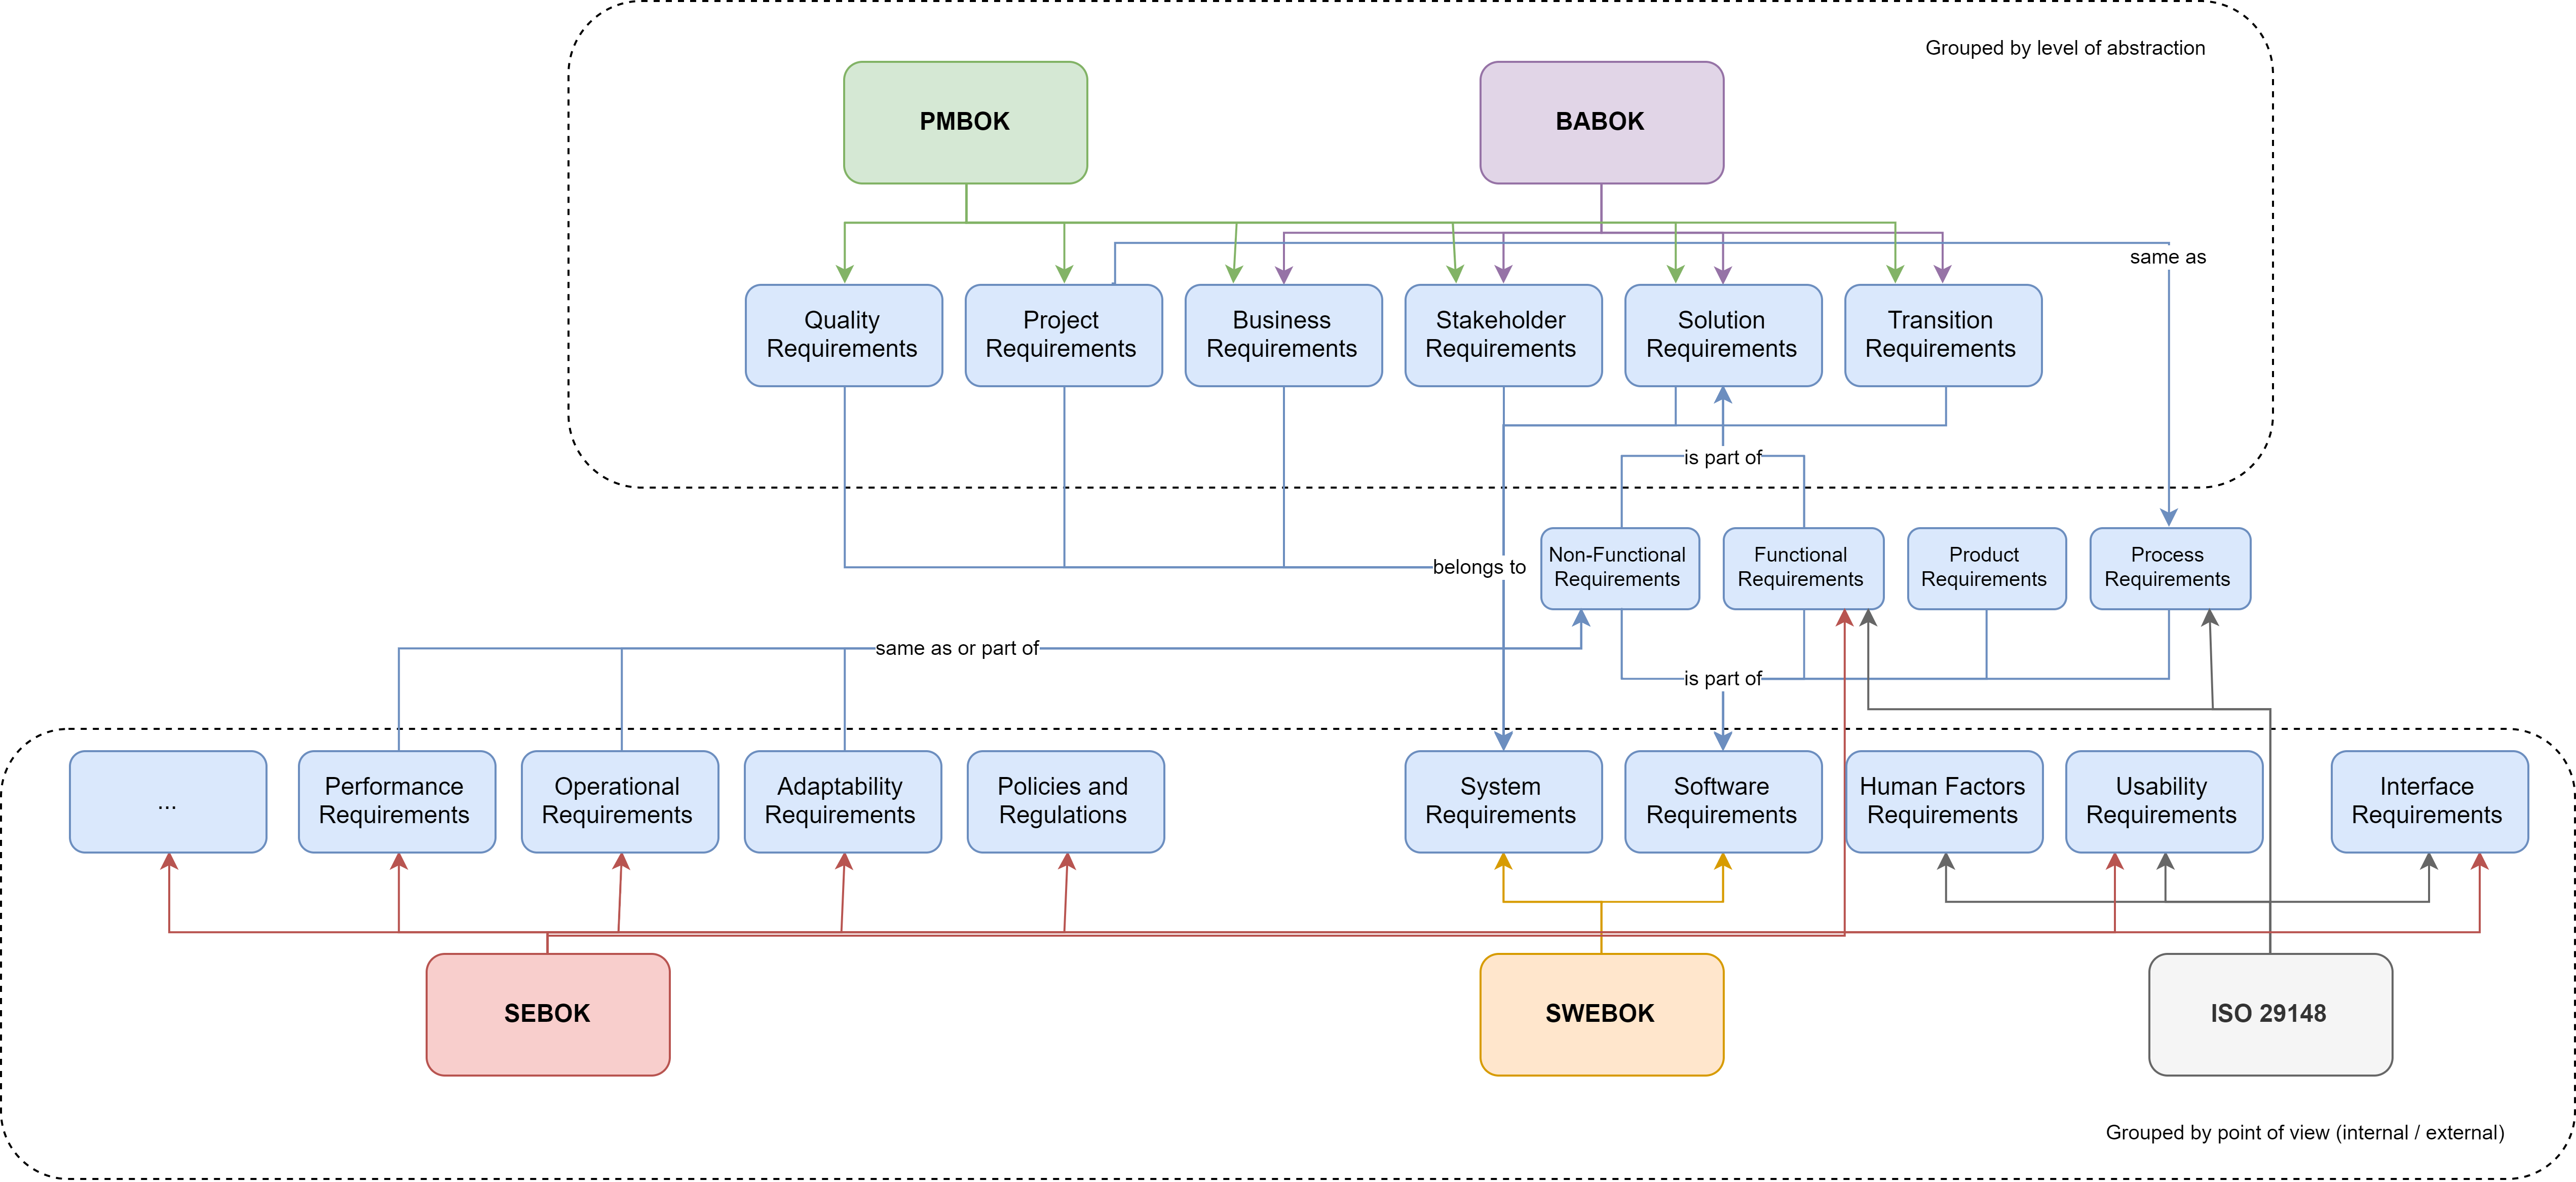
\includegraphics[width=1.0\textwidth]{gfx/Requirements.png}
 \caption{Einordnung der Begriffe und Zusammenhänge unterschiedlicher Normen und Standards}
 \label{fig:chapter05:requirements}
\end{figure}

Das Schaubild \ref{fig:chapter05:requirements} zeigt die unterschiedlichen Normen und Standards grafisch auf und stellt die verschiedenen Anforderungsgruppierungen zueinander in Beziehung.

Grundsätzlich unterscheiden die vorgestellten Ansätze zur Anforderungsklassifizierung zwei Sichtweisen: \ac{PMBOK} und \ac{BABOK} unterscheiden Anforderungen nach Abstraktionslevel während \ac{SWEBOK}, \ac{SEBOK} und ISO29148 primär nach der Perspektive der Stakeholder gruppieren. Das Schaubild \ref{fig:chapter05:requirements_grouping} stellt diesen Zusammenhang grafisch dar.

\begin{figure}[htbp]
 \centering
 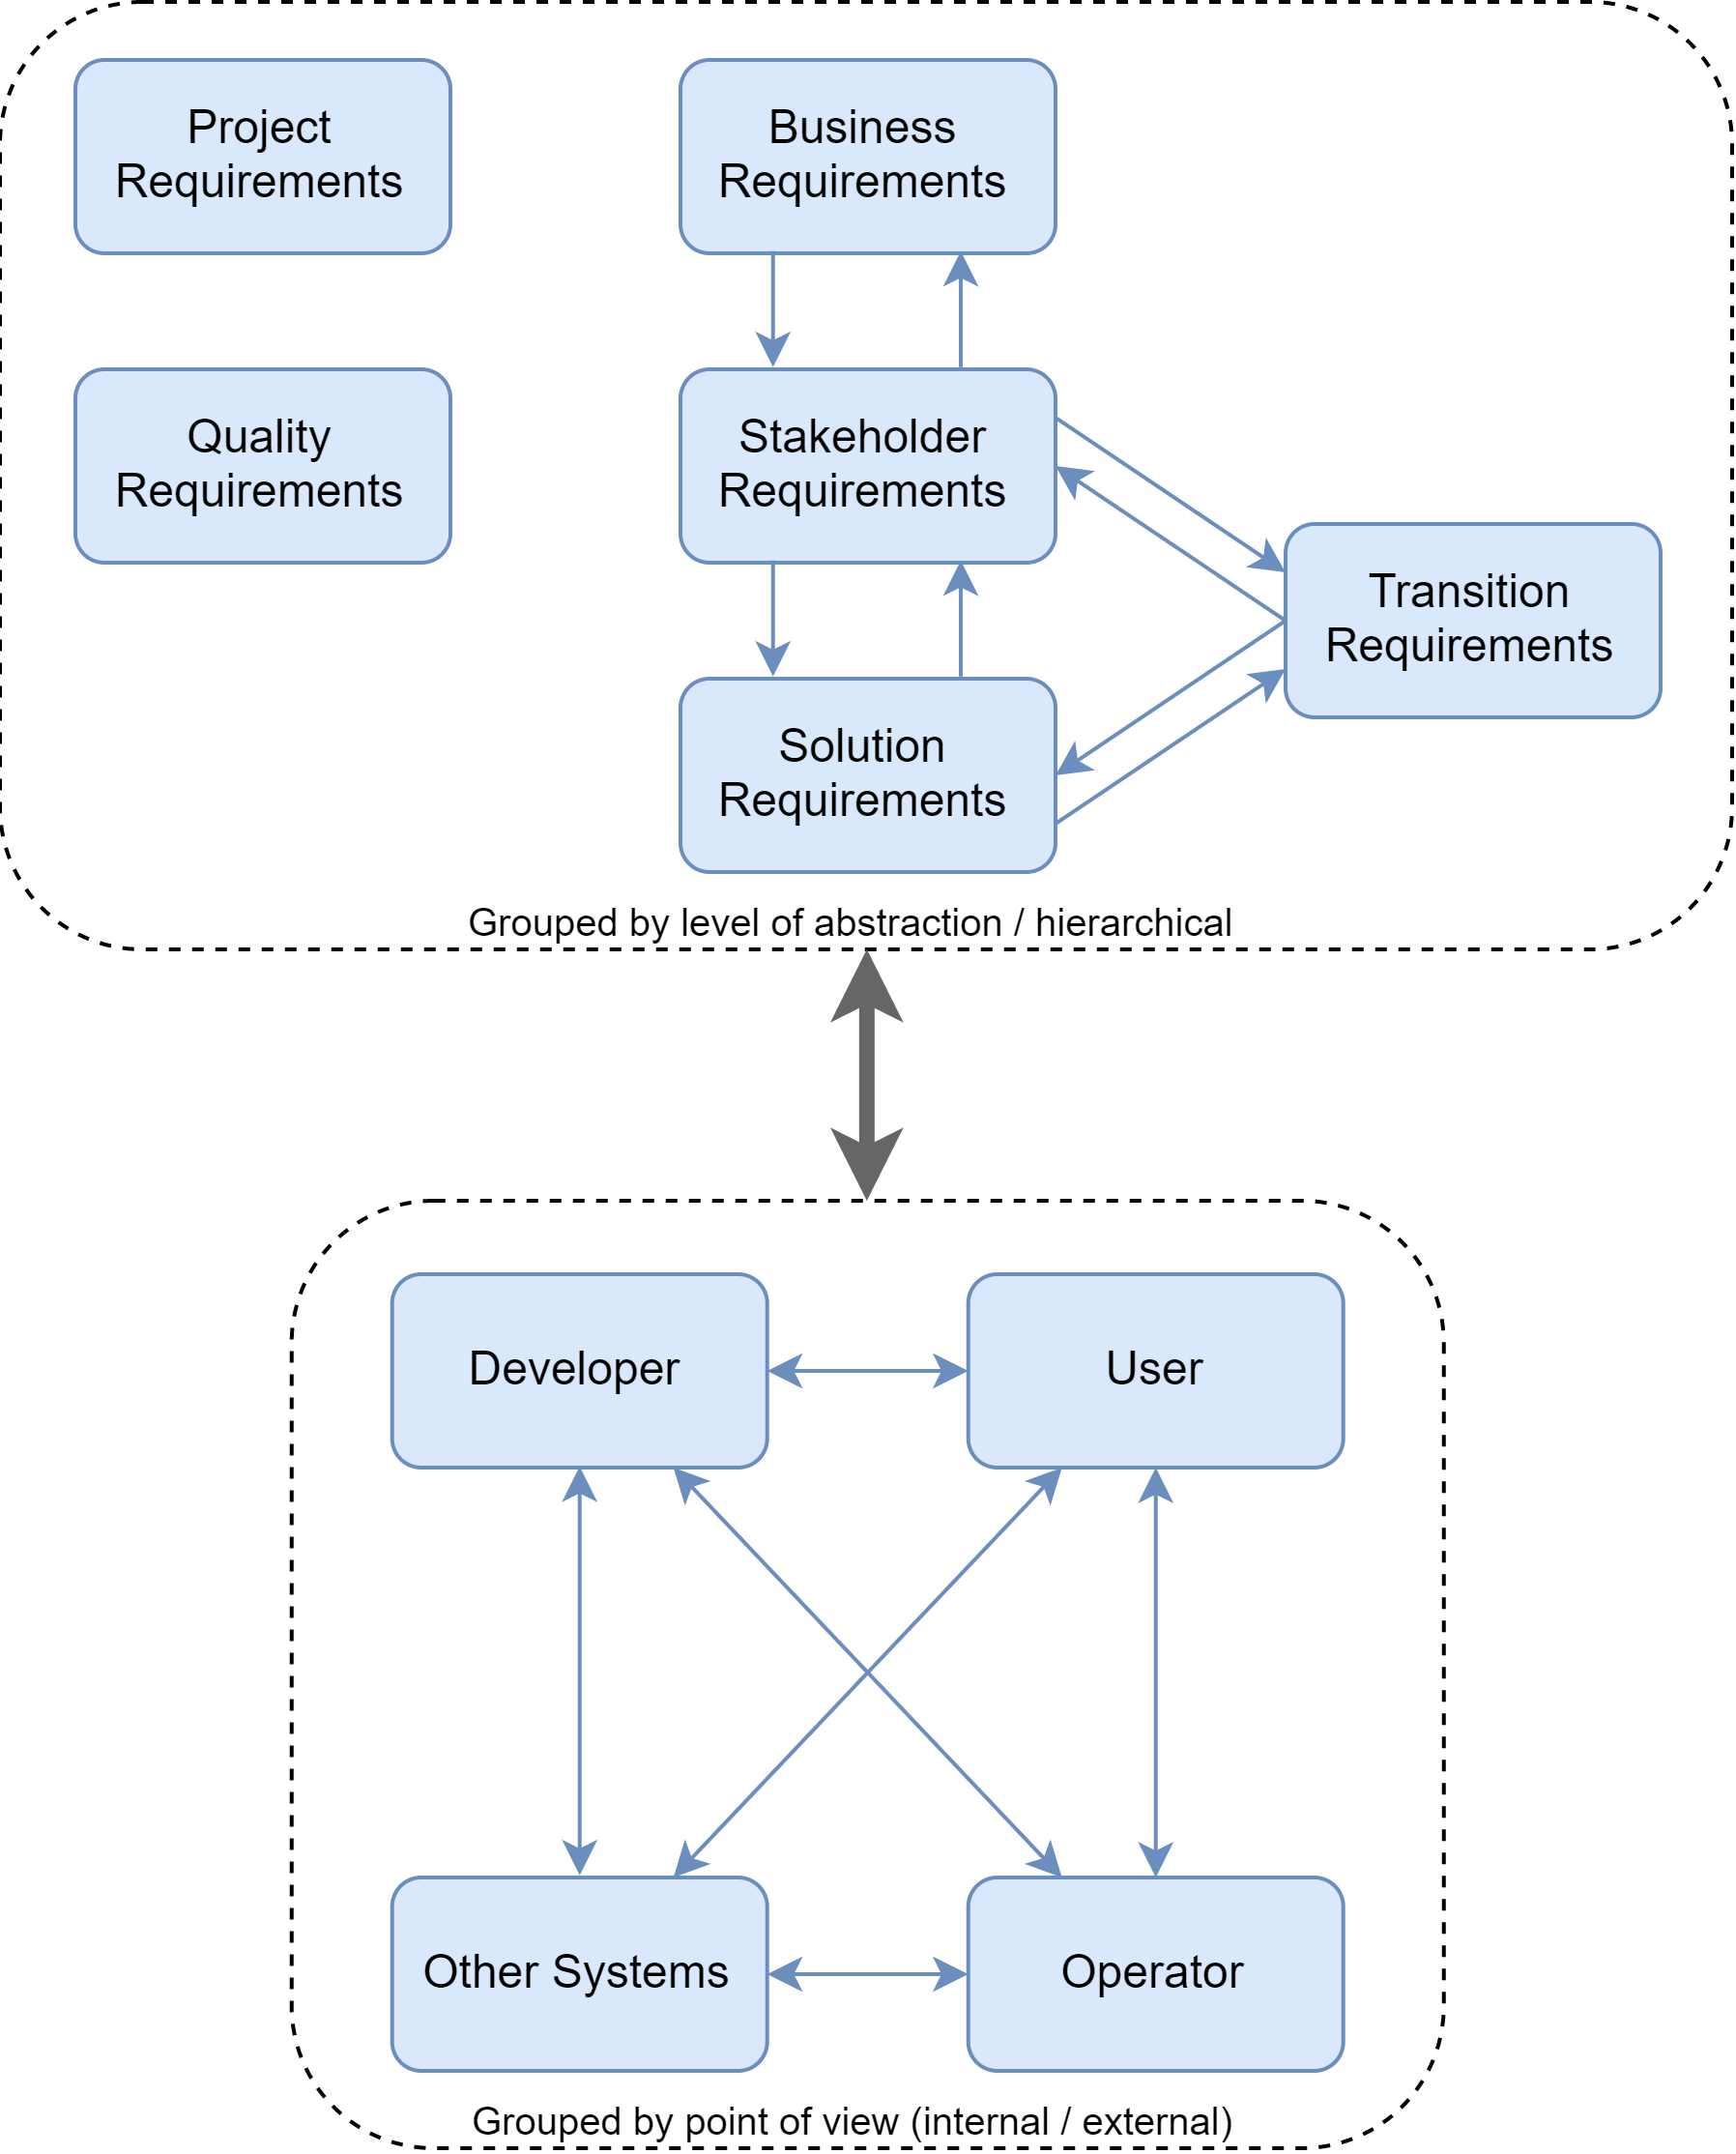
\includegraphics[width=1.0\textwidth]{gfx/Requirements_Grouping.png}
 \caption{Anforderungen werden nach zwei verschiedenen Ansätzen gruppiert.}
 \label{fig:chapter05:requirements_grouping}
\end{figure}

\section{Ableitung eines Klassifizierungsmodells}
\label{sec:requirements:model}
Die Vorteile mehrerer der vorgstellten Ansätze zur Anforderungsklassifizierung können kombiniert werden, indem Anforderungen stufenweise in Unterklassen unterteilt werden. Dabei wird sich der Klassifizierung des \cite{SWEBOK}, \cite{PMBOK} bzw. \cite{BABOK} und \cite{ISO25010} bedient und die folgende Einordnung erstellt:

\begin{description}
  \item[System-Anforderungen] Anforderungen dieser Klasse beziehen sich auf das Gesamtsystem.\\
  \item[Software-Anforderungen] Anforderungen dieser Klasse beziehen sich auf die Softwarekomponente des Gesamtsystems.\\
  \item[Business-Anforderungen] Diese Anforderungen gehören zu der Klasse der System-Anforderungen und beschreiben Anforderungen, die sich an das Geschäftsmodell hinter dem Gesamtsystem richten. Der Scherpunkt liegt auf dem Mehrwert für die Organisation und dem damit verbundenen Nutzen des Gesamtsystems.\\
  Leitfrage: \glqq Welche Geschäftsfälle gibt es und wie werden diese abgedeckt? Welche Richtlinien und Vorgaben müssen beachtet werden? \grqq
  \item[Stakeholder-Anforderungen] Diese Anforderungen gehören zu der Klasse der System-Anforderungen und beschreiben Anforderungen, die die Interessen der beteiligten Stakeholder widerspiegeln und sich keiner anderen Klasse zuordnen lassen.\\
  Leitfrage: \glqq Was muss das Gesamtsystem aus Sicht von [Stakeholder] können? \grqq
  \item[Transition-Anforderungen] Diese Anforderungen gehören zu der Klasse der System-Anforderungen und beschreiben den Übergang vom IST-Zustand des Systems in den SOLL-Zustand. Beispiele hierfür sind benötigte Anwenderschulungen oder Datenkonvertierungen.\\
  Leitfrage: \glqq Was muss gegeben sein, damit sich das Gesamtsystem von Zustand A in den Zustand B überführen lässt? \grqq
  \item[Projekt-Anforderungen] Diese Anforderungen gehören zu der Klasse der System-Anforderungen und beschreiben die Rahmenbedingungen an das Entwicklungsprojekt. Beispiele hierfür können die Projektsprache und Dokumentationsrichtlinien sein.\\
  Leitfrage: \glqq Welche Rahmenbedingungen sind dem Entwicklungsprojekt gegeben? \grqq
  \item[Qualität-Anforderungen] Als Unterklasse der System-Anforderungen beschreiben die Qualität-Anforderungen die Qualitätsansprüche an das System und die Entwicklung und definieren Akzeptanzkriterien ähnlich zu \ac{DoR} bzw. \ac{DoD}.\\
  Leitfrage: \glqq Welche Qualitätsansprüche werden an das Gesamtsystem gestellt? \grqq
  \item[Nicht-funktionale Anforderungen] Diese Anforderungen werden gemäß \ac{ISO}-Norm 25010 zur Software-Qualität definiert und sind Teil der Software-Anforderungen. Dazu zählen zum Beispiel die Performanz, die Kompatibilität und die Benutzbarkeit. Eine ausführliche Auflistung aller Klassen unter dem Sammelbegriff der nicht-funktionalen Anforderungen sowie die genauen Definitionen der Begriffe kann unter \cite{ISO25010} eingesehen werden.\\
  Leitfrage: \glqq Wie gut muss die Software etwas können? \grqq
  \item[Funktionale Anforderungen] Diese Unterklasse der Software-Anforderungen beschreibt, was das Software-System leisten muss und welche Aufgaben es erfüllen muss.\\
  Leitfrage: \glqq Was muss die Software können? \grqq
  \item[Prozess-Anforderungen] Als Untergruppe der Software-Anforderungen bündelt diese Klasse alle Anforderungen, die den Prozess beschreiben, damit die Software so wird, wie gefordert. Typischerweise sind Anforderungen an den Softwareentwicklungsprozess enthalten.\\
  Leitfrage: \glqq Was ist beim Entwickeln der Software zu beachten? \grqq
  \end{description}

Die Abbildung \ref{fig:chapter05:requirements_hierarchy} fasst die Anforderungstypen zusammen und stellt sie hierarchisch strukturiert dar. Es wird deutlich, dass das entwickelte Modell beide Sichtweisen (vgl. Abbildung \ref{fig:chapter05:requirements_grouping}) aufgreift. Auf Seite der System-Anforderungen werden verschiedene Abstraktionslevel wie zum Beispiel die Business-Anforderungen und die Stakeholder-Anforderungen unterschieden. Stakeholder-Anforderungen wiederum spiegeln die Interessen der Beteiligten wider und betrachten die Anforderungen zusammen mit den Software-Anforderungen aus unterschiedlichen Perspektiven.

\begin{figure}[htbp]
 \centering
 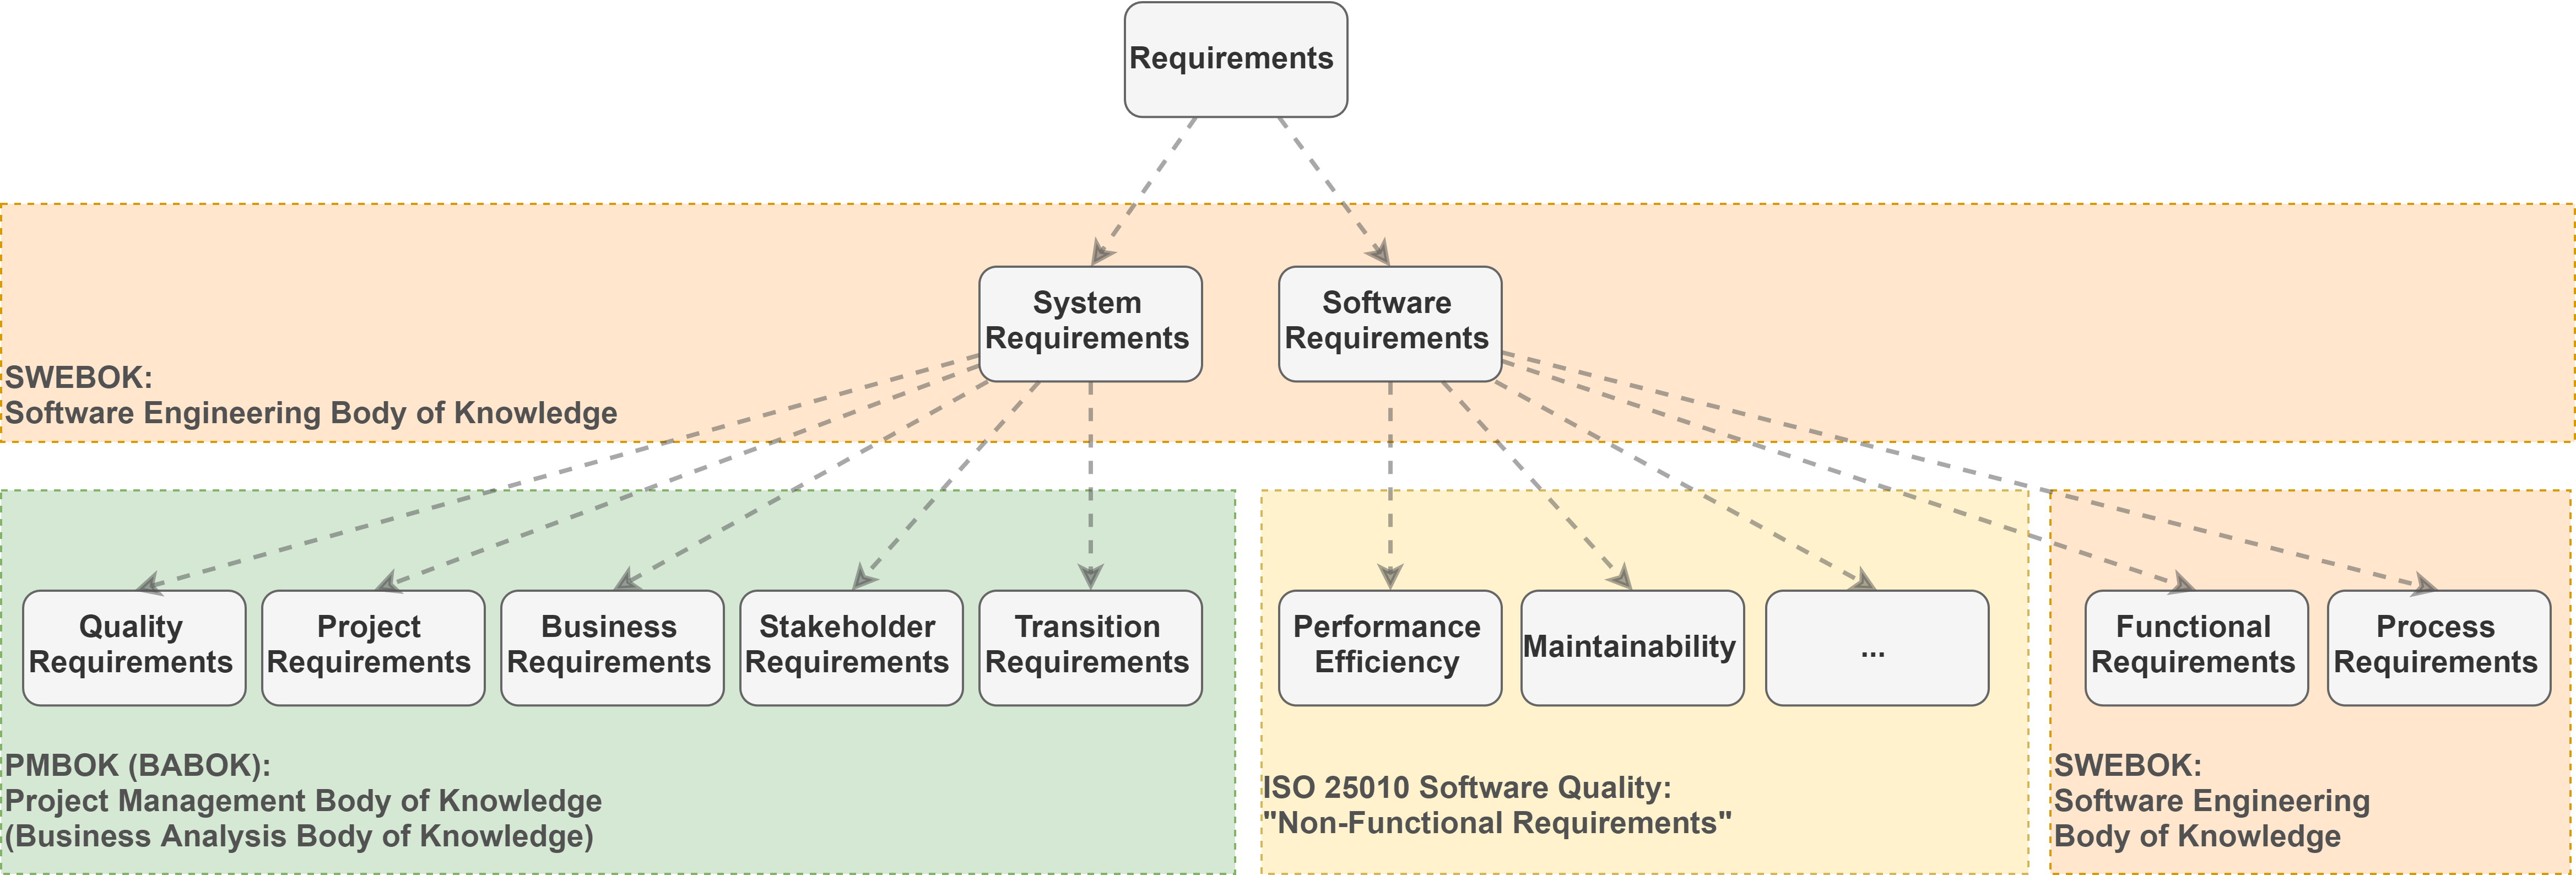
\includegraphics[width=1.0\textwidth]{gfx/Requirements_Hierarchy.png}
 \caption{Anforderungsklassifizierung als kombiniertes Modell aus \cite{SWEBOK}, \cite{PMBOK} bzw. \cite{BABOK} und \cite{ISO25010}}
 \label{fig:chapter05:requirements_hierarchy}
\end{figure}

%
% Section: Anforderungsanalyse
%
\section{Anforderungsanalyse}
\label{sec:requirements:analysis}
In diesem Abschnitt werden die Anforderungen zu dem in Kapitel \ref{ch:iot_usecase} vorgestellten Anwendungsfall ermittelt. Dazu werden zunächst alle beteiligten Stakeholder identifiziert und kurz beschrieben. Anschließend werden aus der jeweiligen Perspektive heraus User-Stories gebildet und die daraus abgeleiteten Tasks aufgelistet. Eine detaillierte Beschreibung aller daraus resultierenden Anforderungen sowie die genaue Zuordnung zu den User-Stories sind im Anhang \ref{ch:appendix:requirements} zu finden.\\

Die Rollen Hersteller, Kunde, Service-Dienstleister und Lieferant wurden bereits unter \ref{description:chapter04:stakeholder} beschrieben. Die folgende Auflistung zeigt weitere Anforderungsrollen, die über die bereits genannten hinausgehen:
\begin{description}
  \item[Plattform-Betreiber] Der Plattform-Betreiber ist verantwortlich für den Betrieb der Plattform und ist hauptsächlich an einem stabilen System und einer einfachen Wartung der Software interessiert.
  \item[IT-Security-Beauftragter] Für den IT-Security-Beauftragten stehen alle sicherheitsrelevanten Themen im Fokus. Dazu zählen insbesondere Verschlüsselung, Datensicherheit und Datenschutz sowie die Authentizität von Daten.
  \item[Business-Developer] Der Business-Developer beschäftigt sich mit der Unternehmensentwicklung und hat Anforderungen an das Geschäftsmodell, die Wirtschaftlichkeit und die Zielerreichung des Gesamtsystems.
  \item[System-Architekt] Für den Software-Architekten stehen alle Fragen rund um die IT-Architektur der Plattform im Vordergrund. Dazu zählen \acp{API}, Modularisierung und der generelle Aufbau der Software.
\end{description}

Um konkrete Anforderungen zu erstellen, werden Userstories aus der Perspektive jedes Stakeholders erarbeitet. Userstories beschreiben eine Funktionalität des Systems, welche aus Sicht der jeweiligen Rolle benötigt wird, um ein bestimmtes Ziel zu erreichen oder einen bestimmten Zweck zu erfüllen. Somit haben alle Userstories die einheitliche Grundstruktur:\\
\begin{quote}
  \glqq Als [Rolle] möchte ich [Funktion], um [Ziel / Zweck] zu erreichen.\grqq
\end{quote}
Zu jeder User-Story werden Tasks beschrieben, die die User-Stories in logische Teile untergliedern. Im letzten Schritt werden diese Tasks feingranular in Anforderungen unterteilt. Die Klassifizierung wird anschließend nach dem erarbeiteten Modell aus \ref{sec:requirements:model} durchgeführt.\\

Die erste Userstory (A1) fasst grundlegende Tätigkeiten über das Agieren auf der Plattform als Akteur (Hersteller, Kunde, Service-Dienstleister, Lieferant, Endgerät) zusammen. Dies beinhaltet sämtliche Interaktionen und Bedingungen, die für alle Akteure gleich sind. Die Userstory A1 beinhaltet vier Tasks:
\begin{itemize}
  \item Die Zugangsberechtigung zur Plattform ist in fünf Anforderungen untergliedert, vier davon sind als \textit{Funktionale Anforderungen} klassifiziert, eine als \textit{Security Anforderung}.
  \item Die Kommunikation zwischen Rollen ist durch fünf Anforderungen definiert und beinhaltet eine \textit{Funktionale Anforderung}, drei \textit{Security Anforderungen} und eine \textit{Performance-Efficiency Anforderung}.
  \item Die Vertragsgestaltung ist in in elf Tasks untergleidert, zwei davon sind \textit{Security}, neun \textit{Funktionale Anforderungen}.
  \item Grafische Oberflächen, die alle Akteure zur Interaktion mit der Plattform benötigen, sind in zwei \textit{Funktionale Anforderungen} unterteilt.
\end{itemize}

Userstories M1 bis M3 stellen die Anforderungen aus Sicht eines Manufacturers dar:
\begin{itemize}
  \item Userstory M1 beschreibt die Vermietung von Endgeräten und beinhaltet zwei Tasks mit insgesamt sechs Anforderungen. Fünf der sechs Anforderungen sind \textit{Funktionale Anforderungen}, eine wurde als \textit{Portability Anforderung} klassifiziert.
  \item Userstory M2 beschreibt das Erzeugen von Verträgen und beinhaltet einen Task mit drei Anforderungen, welche alle der Klasse der \textit{Funktionalen Anforderungen} zugeordnet wurden.
  \item Userstory M3 beschreibt die Abrechnung von Verträgen und beinhaltet zwei Tasks mit insgesamt drei Anforderungen, wobei eine Anforderung als \textit{Funktionale Anforderung}, eine als \textit{Performance-Efficiency Anforderung} und eine als \textit{Security Anforderung} bestimmt wurde.
\end{itemize}

Die Userstories C1 bis C3 zeigen die Sicht des Customers:
\begin{itemize}
  \item Userstory C1 beschreibt die Ansicht verfügbarer Geräte, also eine Oberfläche, die dem Customer bereitgestellt werden muss, auf der er alle zur Miete verfügbaren Geräte gelistet bekommt. Diese Userstory beinhaltet zwei Tasks mit insgesamt zwei \textit{Funktionalen Anforderungen}.
  \item Userstory C2 beschreibt die Wartung und Reinigung der Geräte durch den Customer und beinhaltet vier Tasks mit insgesamt sechs Anforderungen. Dabei handelt es sich um vier \textit{Funktionale Anforderungen}, eine \textit{Security Anforderung} und eine \textit{Performance-Efficiency Anforderung}.
  \item Userstory C3 beschreibt die Bedienbarkeit aus Nutzersicht und beinhaltet zwei Tasks mit insgesamt drei Anforderungen. Dabei handelt es sich um eine \textit{Transition Anforderung} und zwei \textit{Usability Anforderungen}.
\end{itemize}

Die Userstories SP1 und SP2 sind aus Sicht des Service-Providers beschrieben:
\begin{itemize}
  \item Userstory SP1 beschreibt das Anbieten eigener Service-Dienstleistungen auf der Plattform mit einem Task und zwei \textit{Funktionalen Anforderungen}.
  \item Userstory SP2 beschreibt das Abschließen von Service-Aufträgen nach getätigtem Service an den Geräten vor Ort und ist unterteilt in zwei Tasks mit je zwei \textit{Funktionalen Anforderungen}.
\end{itemize}

Die Userstories SEC1 bis SEC3 sind aus Sicht des Security-Beauftragten beschrieben:
\begin{itemize}
  \item Userstory SEC1 beschreibt die sichere Zahlungsabwicklung und ist in zwei Tasks mit insgesamt fünf Anforderungen unterteilt. Dabei handelt es sich um zwei \textit{Funktionale Anforderungen} und drei \textit{Security Anforderungen}.
  \item Userstory SEC2 beschreibt die sichere Kommunikation mittels signierter Nachrichten und untergliedert sich in zwei Tasks mit insgesamt zwei \textit{Quality Anforderungen}.
  \item Userstory SEC3 beschreibt die Manipulationssicherheit und ist in zwei Tasks mit insgesamt drei \textit{Security Anforderungen} unterteilt.
\end{itemize}


Die Userstories BD1 bis BD4 sind aus Sicht des Business-Developers beschrieben:
\begin{itemize}
  \item Userstory BD1 beschreibt das Geschäftsmodell und beinhaltet zwei Tasks mit insgesamt sechs Anforderungen, wobei fünf davon als \textit{Funktionale Anforderungen} und eine als \textit{Business Anforderung} klassifiziert wurden.
  \item Userstory BD2 beschreibt den Zugang von Geschäftspartnern zu der Plattform und ist in zwei Tasks mit insgesamt drei Anforderungen untergliedert. Diese wurden als \textit{Business Anforderung}, \textit{Transition Anforderung} und \textit{Stakeholder Anforderung} klassifiziert.
  \item Userstory BD3 beschreibt die Plattform als Hersteller-übergreifend und ist in drei Tasks mit insgesamt drei Anforderungen unterteilt. Dabei wurden eine Anforderung als \textit{Business Anforderung} und zwei als \textit{Compatibility Anforderungen} klassifiziert.
  \item Userstory BD4 beschreibt die Abrechnungsmodelle der Plattform und ist in einen Task mit zwei Anforderungen unterteilt. Dabei handelt es sich um eine \textit{Business Anforderung} und einer \textit{Maintainability Anforderung}.
\end{itemize}

Die Userstories SA1 und SA2 sind aus Sicht des System-Architekten beschrieben:
\begin{itemize}
  \item Userstory SA1 beschreibt die einfache Einbindung der Plattform in bestehende Infrastruktur und enthält einen Task mit einer \textit{Process Anforderung}.
  \item Userstory SA2 beschreibt die Robustheit des Gesamtsystems bei Ausfällen und ist in zwei Tasks mit je zwei Anforderungen unterteilt. Dabei handelt es sich um zwei \textit{Security Anforderungen} und zwei \textit{Reliability Anforderungen}.
\end{itemize}

Die Userstory P1 ist aus Sicht des Plattform-Betreibers beschrieben:
\begin{itemize}
  \item Userstory P1 beschreibt die automatisierte Bereitstellung der Software und ist in zwei Tasks mit je einer Anforderung untergliedert. Diese sind als \textit{Maintainability Anforderung} und als \textit{Portability Anforderung} klassifiziert.
\end{itemize}

Insgesamt wurden 19 Userstories beschrieben, die in 39 Tasks unterteilt wurden. Die 83 daraus resultierenden Anforderungen wurden klassifiziert, sodass sich 9 Level-1 \textit{System-Anforderungen} und 74 Level-1 \textit{Software-Anforderungen} ergaben. Für jede Level-2 Klasse unterhalb der \textit{System-Anforderungen} wurden Anforderungen ermittelt - bis auf die Klasse der Projekt-Anforderungen. Im Rahmen dieser Arbeit wird ein \ac{PoC} entwickelt, womit diese Arbeit aus Sicht der Anforderungserstellung als Entwicklungsprojekt angesehen werden kann. Rahmenbedingungen wie die zeitliche Begrenzung des Projektes oder den Reifegrad eines \acp{PoC} könnten als Projekt-Anforderungen definiert werden. Da dies aber keine konkrete Auswirkung auf den Anwendungsfall als solchen hat, wird an dieser Stelle auf diese Klasse verzichtet. Bei der Entwicklung eines marktreifen Produktes in einem realen Entwicklungsprojekt ist diese Klasse allerdings zu beachten.\\
Auf Seiten der Software-Anforderungen werden alle Level-2 Klassen abgedeckt. Die Subklasse \textit{Functionality-Suitability Anforderungen} erhält im Modell eine eigene Klasse, da es sich um Funktionale Anforderungen handelt.

%
% Section: Anforderungsevaluierung
%
\section{Anforderungsevaluierung}
\label{sec:requirements:evaluation}
Die Anforderungsevaluierung hat zum Ziel, die im vorherigen Abschnitt beschriebenen und klassifizierten Anforderungen schrittweise zu reduzieren, um die \ac{DLT}-relevanten Anforderungen zu identifizieren. Dabei handelt es sich um Anforderungen, die relevant für eine technische Umsetzung auf Basis einer \ac{DLT}-Lösung sind.\\
Um die Relevanz für den Kontext \ac{DLT} festzustellen, wurde die Anforderungsliste mit den Fachexperten der Abteilung für Distributed Ledger Technologies der Firma MaibornWolff GmbH in mehreren Diskussionsrunden durchgearbeitet und nach Einschätzung der Experten entsprechend gewertet.


\subsection{System-Anforderungen}
\label{subsec:requirements:evaluation:system}
Die erste Level-2 Subklasse der \textit{System-Anforderungen} ist die Klasse der \textit{Quality Anforderungen}. Diese Klasse definiert die Qualitätskriterien, die die Plattform erfüllen muss. Anforderungen dieser Klasse fungieren oft als Enabler für weitere Anforderungen anderer Klassen. Für den beschriebenen IOT-Anwendungsfall wurden zwei Anforderungen identifiziert, die dieser Klasse zuzuordnen (Anforderungen SEC2.1.1, SEC2.2.1) und Teil der Userstory SEC2 sind. Sie beschreiben, dass die Verwendung von HTTPS bzw. SSL/TLS ein vorgeschriebenes Qualitätskriterium ist. Darüber hinaus müssen Passwortregeln hinterlegbar sein, um die Sicherheit der auf der Plattform verwendeten Passwörter zu gewährleisten. Es wird deutlich, dass die Anforderungen dieser Klasse primär Rahmenbedingungen darstellen und keine direkten Auswirkungen auf die technische Basis haben. Diese Qualitätsansprüche, die mit den genannten Anforderungen einhergehen, haben keine Auswirkung auf eine mögliche Umsetzung der Plattform durch eine \ac{DLT}-Lösung. Damit werden die Anforderungen im weiteren Verlauf nicht tiefergehend betrachtet.\\

Die zweite Level-2 Subklasse der \textit{System-Anforderungen} ist die Klasse der \textit{Project Anforderungen}, die Rahmenbedingungen an das Projekt beschreiben. Die Entwicklung des \ac{PoC} im Rahmen dieser Arbeit stellt ein solches Entwicklungsprojekt dar, ist allerdings für die Betrachtung in diesem Kontext hinsichtlich \ac{DLT}-Relevanz nicht weiter zu berücksichtigen. Die \textit{Project Anforderungen} werden entsprechend nicht in die weitere Analayse miteinbezogen.\\

Die dritte Level-2 Subklasse der \textit{System-Anforderungen} ist die Klasse der \textit{Business-Anforderungen}, die die Geschäftsfälle und -anforderungen von einer abstrakteren Perspektive betrachten. Im Fokus stehen die Bedürfnisse und Rahmenbedingungen des Unternehmens, welches die Plattform beauftragt hat. Im Rahmen des IOT-Anwendungsfalls wurden vier Anforderungen dieser Klasse identifiziert (Anforderungen BD1.1.1, BD2.1.1, BD3.1.1 und BD4.2.1); betroffen sind die Userstories BD1 bis BD4. Die Anforderungen decken das Abrechnungsmodell Pay-As-You-Use ab und beschäftigen sich mit der aktuellen und zukünftigen geschäftlichen Ausrichtung der Plattform. Letzteres hat keine Auswirkungen auf die technische Basis, die die zugrundeliegende Plattform verwendet: Es handelt sich um keine Technologie-entscheidende Anforderung. Anforderung BD4.2.1 beschreibt, dass ein Pay-As-You-Use Abrechnungsmodell in einem Vertrag abgebildet wird. Diese Anforderung ist \ac{DLT}-relevant: Zum einen impliziert diese Anforderung, dass eine zugrundeliegende \ac{DLT}-Plattform in der Lage ist, Verträge abzubilden: Im Umfeld von \acp{DLT} bietet sich die Abwicklung der Vertragslogik mittels Smart-Contracts an. Zum anderen muss gewährleistet sein, dass die Smart-Contract Implementierung mächtig genug ist, um das Abrechnungsmodell Pay-As-You-Use codieren zu können. Diese Anforderung muss in die weitere Analyse miteinbezogen werden.\\

Die vierte Level-2 Subklasse der \textit{System-Anforderungen} ist die Klasse der \textit{Stakeholder-Anforderungen}, welche Anforderungen speziell aus der Sicht einzelner Stakeholder beschreiben, die mit anderen Klassen noch nicht abgedeckt werden konnten. Im Kontext des Anwendungsfalls wurde eine Anforderung identifiziert (BD2.2.1), die dieser Klasse zuzuordnen ist und zur Userstory BD2 gehört. Es wird der Onboarding-Prozess eines Geschäftspartners beschrieben, indem dieser als Partner identifiziert werden muss. Dieser Prozess muss entsprechend der Anforderungen gestaltet werden, womit es sich um eine abstrakte Beschreibung dessen, wie ein Prozess auszusehen hat, handelt. Es werden keine technischen Details gefordert, wodurch keine Abhängigkeiten zu der technischen Umsetzung der Plattform entstehen. Damit ist diese Klasse für die weitere Analyse nicht relevant und kann vernachlässigt werden.\\

Die fünfte Level-2 Subklasse der \textit{System-Anforderungen} ist die Klasse der \textit{Transition Anforderungen}, die sämtliche Anforderungen von einem IST-Zustand (zeitlich vor der Einführung der Plattform) in einen SOLL-Zustand (zeitlich nach Einführung der Plattform) beinhaltet. Zwei Anforderungen (Anforderungen C3.1.1 und BD2.1.2) wurden identifiziert, die dieser Klasse zuzuordnen und Teil der Userstories C3 und BD2 sind. Es handelt sich in dem vorliegenden Kontext um Anforderungen, die die schnelle Erlernbarkeit durch den Benutzer sowie die Schulung von Mitarbeitern zur Nutzung der Plattform beschreiben und somit die \ac{UX} in den Vordergrund stellen. Da es sich in diesem Fall um Aufbau, Verständlichkeit und Benutzbarkeit einer grafischen Oberfläche (Schnittstelle zum Benutzer) handelt, kann diese Klasse ebenfalls vernachlässigt werden.\\

\subsection{Software-Anforderungen}
\label{subsec:requirements:evaluation:software}
Anforderungen dieser Level-1 Klasse stellen den Großteil aller Anforderungen dar. In einem realistischen Entwicklungsprojekt sind die individuellen Rahmenbedingungen, Qualitätskriterien, Business-Richtlinien und Integrationsrichtlinien des jeweiligen Unternehmens zu beachten. Die in dieser Arbeit aufgestellten System-Anforderungen decken nur die grundlegendsten Anforderungen dieser Kategorie ab. Die \textit{Software-Anforderungen}, die in diesem Abschnitt evaluiert werden, sind unabhängig von den \textit{System-Anforderungen} stets dieselben.\\

Die erste Level-2 Subklasse der \textit{Software-Anforderungen} sind die \textit{Process Anforderungen}, die Anforderungen an den Entwicklungsprozess der Software stellen. Für den vorliegenden IOT-Anwendungsfall wurde eine Anforderung (SA1.1.1) ermittelt, die zu der Userstory SA1 gehört. Während der Entwicklung ist darauf zu achten, dass die Modularität der Softwarekomponenten gewahrt bleibt, damit diese später unabhängig voneinander bereitgestellt und gewartet werden können. Dies hat keine Auswirkung auf die Umsetzung auf Basis einer \ac{DLT}-Lösung. Im Allgemeinen haben Anforderungen dieser Klasse einerseits eine technische Relevanz, da sie zum Beispiel einzusetzende Technologien für Schnittstellen beschränken oder die Art und Weise definieren, wie Software entwickelt werden soll. Andererseits kann jede Software durch den Einsatz einer geeigneten Middleware miteinander verbunden werden, sollten vorhandene Schnittstellen und Softwarekomponenten nicht Standard-konform oder kompatibel sein. Somit können die Anforderungen dieser Klasse ebenfalls vernachlässigt werden.\\

Die zweite Level-2 Subklasse der \textit{Software-Anforderungen} sind die \textit{Funktionalen Anforderungen}, die beschreiben, welche Funktionalität die Plattform anbieten muss. Für den vorliegenden IOT-Anwendungsfall wurden 46 solcher Anforderungen ermittelt, die insgesamt zehn Userstories betreffen. Um die Übersichtlichkeit zu bewahren, wurde diese Klasse in verschiedene, logische Abschnitte gegliedert. Diese wurden nach der inhaltlichen Thematik der Anforderungen definiert und folgen keiner speziellen Klassifizierung.

\begin{description}
  \item[GUI] 12 der 46 Anforderungen dieser Klasse betreffen direkt oder indirekt die grafische Darstellung für den Benutzer. Es handelt sich hierbei lediglich um das Frontend, welches Daten aufbereitet darstellt und Schaltflächen zur Interaktion mit dem Backend bereitstellt. Somit werden die Anforderungen dieser Klasse für weiterführende Analysen nicht beachtet. Konkret handelt es sich um die Anforderungen A1.1.4, A1.3.4, A1.4.1, A1.4.2, M2.1.1, M2.1.2, M2.1.3, C1.1.1, C1.2.1, SP1.1.1, SP1.1.2 und SP2.2.1.

  \item[Endgerät] 15 der 46 Anforderungen beziehen sich auf Funktionalitäten, die das Endgerät bereitstellen muss, um auf der Plattform vermietet werden zu können. Dabei geht es primär um die Konnektivität zu der Plattform, die Funktionsweise der verbauten Sensoren sowie der Kommunikation mit dem Customer und dem Service-Provider. Die Endgeräte fungieren in ihrer Rolle als Peripherie; es kann sich um Haushaltsgeräte aller Art handeln - von der Kaffeemaschine bis zur Waschmaschine. Die Schnittstellen hin zur Plattform sind klar definiert. Auf der einen Seite wird deutlich, dass die meisten Anforderungen an die Geräte unabhängig von der technischen Umsetzung der Plattform sind und keinen Einfluss auf deren Umsetzung haben. Bei Inkompatibilität eines Endgeräts zur Plattform wäre der Einsatz einer Middleware sinnvoll, die die Integration zur Plattform sicherstellen könnte. Eine Möglichkeit wäre die Verwendung eines lokalen Gateways, das die Daten der Geräte konvertiert und an die Plattform übermittelt. Standardmäßig sollten die Geräte die Kommunikation mit der Plattform bereits Hersteller-seitig gewährleisten. Auf der anderen Seite spielt gerade die Konnektivität eine ganz entscheidende Rolle: Die Tatsache, dass Endgeräte nicht jederzeit mit der Plattform verbunden sind - bedingt durch Verbindungsprobleme oder Ähnliches - stellt eine zentrale Anforderung an die zugrundeliegende Plattform dar. Um auch im Offline-Modus mit seinem Umfeld interagieren zu können, zum Beispiel um einen Kaffee zu servieren, muss das Gerät zeitnah auf Benutzereingaben reagieren, da ansonsten ein schlechtes Benutzererlebnis entstünde. Würde das Gerät erst dann reagieren, wenn es alle benötigten Informationen von der Plattform erhalten hat, also nachdem es wieder eine Verbindung aufbauen konnte, wäre der Anwendungsfall inpraktikabel und hätte keine wirtschaftliche Daseinsberechtigung. Deshalb muss es möglich sein, dass das Gerät voll funktionsfähig arbeitet, auch wenn es keine Konnektivität zur Plattform hat. Anlaufende Kosten und Informationsengpässe müssen handhabbar sein und zu einem späteren Zeitpunkt synchronisierbar sein. Diese Anforderung hat eine sehr hohe \ac{DLT}-Relevanz und muss für die folgende Analyse genaustens berücksichtigt werden. (Anforderungen M1.1.1, M1.1.2, M1.1.3, M1.2.1, M1.2.2, M1.2.3, M1.2.4, M3.1.1, C2.1.1, C2.1.2, C2.3.1, C2.4.1, SP2.1.1, SP2.1.2 und SP2.2.2)
  \item[Kommunikation] Drei der 46 Anforderungen beziehen sich auf die Kommunikation zwischen Akteuren auf der Plattform (Anforderungen A1.2.1, A1.3.1 und A1.3.3). Anforderung A1.3.1 beschreibt die Kommunikation über Verträge, die die Akteure der Plattform miteinander abschließen können. Im Kontext einer \ac{DLT}-Lösung bedeutet das, dass die Plattform in der Lage sein muss, einen Vertrag abzubilden (siehe Business-Anforderungen oben). Diese Anforderung hat eine \ac{DLT}-Relevanz und muss in der weiteren Analyse betrachtet werden. Die übrig gebliebenen zwei Anforderungen beschreiben allgemeinere Aspekte der Kommunikation auf der Plattform und können vernachlässigt werden.
  \item[Finanzen] Sieben der 46 Anforderungen (A1.3.11, SEC1.1.1, SEC1.1.3, BD1.2.1, BD1.2.2, BD1.2.3 und BD1.2.5) beschreiben den Geldfluss zwischen Akteuren aufgrund ihrer vertraglichen Vereinbarungen. Geldtransfers werden geloggt und vor Ausführung überprüft. Diese Anforderungen sind für eine Umsetzung auf einer \ac{DLT}-Lösung nicht relevant, da sie lediglich die Richtung und Menge des Geldflusses sowie Rahmenbedingungen an Geldtransfers festlegen. Damit allerdings erbrachte Leistungen kostenpflichtig gemäß des Abrechnungsmodells abgerechnet werden können, muss die Plattform zum einen das Abrechnungsmodell implementieren und zum anderen ein digitales Zahlungsmittel bereitstellen. Ersteres kann auf einer \ac{DLT}-Lösung mittels Smart-Contracts umgesetzt werden. Zweiteres bedarf einer internen Währung, um Leistungen nach Verbrauch abzurechnen. Damit sind diese zwei Anforderungen relevant und müssen in der weiteren Analyse beachtet werden.
  \item[Rollenmanagement] Drei der 49 Anforderungen (A1.1.2, A1.1.3 und A1.1.5) definieren das Rollenmanagement und den Zugang zu der Plattform mittels Registrierung und Anmeldung. Letzteres stellt keine Relevanz dar, da es sich um eine standardmäßige Zugangsbeschränkung handelt und nicht abhängig von der Backend-Lösung ist. Im Gegensatz dazu werden Rollen in den Verträgen genutzt, um Berechtigungen der Akteure zu prüfen. Es handelt sich um Informationen, die von Verträgen auf der Plattform einsehbar sein müssen. Content- oder allgemein Informationsprovider, die Informationen auf einer \ac{DLT}-Umgebung bereitstellen, nennt man Oracles (siehe Kapitel \ref{subsec:fundamentals:dlt:smartcontracts}). Hier liegt eine Relevanz in Bezug auf die Umsetzung auf Basis einer \ac{DLT}-Lösung vor und muss im weiteren Verlauf beachtet werden.
  \item[Vertragskonstrukt] Sechs der 49 Anforderungen (A1.3.2, A1.3.6, A1.3.7, A1.3.8, A1.3.10 und BD1.2.4) beschreiben das Vertragskonstrukt: Eigenschaften wie Individualität und Zugriffsregelung haben keinen Einfluss auf die technische Lösung, wohingegen die Komplexität und Editierbarkeit (drei Anforderungen) große Relevanz haben. Zum einen muss die Implementierung eines Vertrages mittels Smart-Contracts auch komplexe Konstrukte abbilden können. Zum anderen sind Smart-Contracts - sind sie einemal in der \ac{DLT} gespeichert - unveränderbar und können als solches nicht überarbeitet werden. Die zugrundeliegende \ac{DLT}-Technologie muss also einen entsprechenden Mechanismus anbieten, um Smart-Contracts zu warten und zu aktualisieren. Darüber hinaus handelt es sich bei den Verträgen, die mittels Smart-Contracts abgebildet werden sollen, um rechtskräftige Miet- und Serviceverträge. Demnach müssen die Implementierungen rechtssicher und rechtskonform abgebildet werden können. Diese Punkte sind bei der Wahl der \ac{DLT}-Lösung zu beachten.
\end{description}


Die dritte Level-2 Subklasse der \textit{Software-Anforderungen} unter dem Sammelbegriff der \textit{Nicht-Funktionalen Anforderungen} heißt \textit{Kompatibilität} (Compatibility). Für den vorliegenden IOT-Anwendungsfall wurden zwei solcher Anforderungen ermittelt (BD3.2.1, BD3.3.1,), welche die Userstory BD3 betreffen. Die Kompatibilität stellt die Fähigkeit des Gesamtsystems dar, Informationen mit anderen System auszutauschen und sich eine Umgebung mit anderen Systemen zu teilen. Es handelt sich hierbei um Anforderungen, die im Kontext des \ac{IOT}-Anwendungsfalls keine Relevanz für die Wahl der technischen Basis haben. Sollten Systeme nicht kompatibel sein, so könnte im Zweifelsfall eine Middleware für die Übersetzung bzw. die Kompatibilität sorgen. Somit werden die Anforderungen dieser Klasse für die weitere Analyse nicht weiter beachtet.


Die vierte Level-2 Subklasse der \textit{Software-Anforderungen} unter dem Sammelbegriff der \textit{Nicht-Funktionalen Anforderungen} nennt sich \textit{Wartbarkeit} (Maintainability). Anforderungen dieser Klasse stellen die Fähigkeit des Gesamtsystems dar, effizient wartbar zu sein um z.B. die Funktionalität zu erweitern und zu verbessern. Konkret im Kontext des \ac{IOT}-Anwendungsfalls beziehen sich die Anforderungen BD4.2.2 und P1.1.1 der zwei Userstories BD4 und P1 auf den Aufbau der Software: Einzelne Module können separat gewartet werden und die Testabdeckung ist hoch genug, damit die Wartung einzelner Module keine unerwünschten Nebeneffekte mit sich führt. Es handelt sich also um generische Anforderungen, die keinen Bezug zur technischen Umsetzung haben und daher keine \ac{DLT}-Relevanz besitzen. Somit wird diese Anforderungsklasse im weiteren Verlauf nicht weiter berücksichtigt.


Die fünfte Level-2 Subklasse der \textit{Software-Anforderungen} unter dem Sammelbegriff der \textit{Nicht-Funktionalen Anforderungen} lautet \textit{Performance-Effizienz} (Performance-Efficiency) und beschreibt die Leistung des Gesamtsystems in Bezug auf die zur Verfügung stehenden Ressourcen. Die Anforderungen dieser Klasse (A1.2.2, M3.2.1 und C2.4.2) im konkreten Anwendungsfall betreffen drei Userstories (A1, M3 und C2) und beschreiben alle das zeitliche Verhalten von übermittelten Daten: Die Kommunikation zwischen Akteuren, Geräten und Verträgen auf der Plattform wird sofort übermittelt. Es werden keine Daten zurückgehalten, aggregiert oder zeitverzögert übermittelt. Diese Anforderungen treffen keine Aussage über die Verarbeitungsdauer der Daten und haben damit keine Relevanz in Bezug auf die Wahl der technischen Basis. Somit werden die Anforderungen dieser Klasse für die weitere Analyse ignoriert.


Die sechste Level-2 Subklasse der \textit{Software-Anforderungen} unter dem Sammelbegriff der \textit{Nicht-Funktionalen Anforderungen} heißt \textit{Portabilität} (Portability) und beschreibt die Fähigkeit des Gesamtsystems von einer Hardware bzw. Umgebung in einer andere migriert zu werden. In diesem Kontext existiert eine Anforderung (P1.2.1) der Userstory P1, welche die automatisierte Installation und Bereitstellung der Software definiert. Hierbei handelt es sich nicht um eine Technologie-entscheidende Anforderung. Demnach wird diese Anforderungsklasse in der weiteren Analyse nicht beachtet.


Die siebte Level-2 Subklasse der \textit{Software-Anforderungen} unter dem Sammelbegriff der \textit{Nicht-Funktionalen Anforderungen} nennt sich \textit{Ausfallsicherheit} (Reliability) und beschreibt, wie gut ein System unter bestimmten Bedingungen die geforderten Funktionalitäten durchführen kann. Anforderung SA2.2.2 definiert, dass die Plattform keinen \ac{SPoF} besitzen darf. Dies zeigt eine generelle Eigenschaft auf und ist im Kontext eines dezentralen Systems wie des \acp{DLT} nicht weiter von Relevanz. Daneben fordert Anforderung SA2.2.1, dass die Plattform in der Lage ist, bis zu 10.000 Endgeräte zu verarbeiten, ohne Einbußen in der Funktionalität oder der Geschwindigkeit der Verarbeitung. Diese Anforderung muss bei der Wahl der zugrundeliegenden \ac{DLT}-Lösung beachtet werden, da hierbei Performanz und Verfügbarkeit beeinträchtigt werden.


Die achte Level-2 Subklasse der \textit{Software-Anforderungen} unter dem Sammelbegriff der \textit{Nicht-Funktionalen Anforderungen} wird als \textit{Sicherheit} (Security) bezeichnet und befasst sich mit der Thematik rund um Software- und Datensicherheit. Diese Klasse beinhaltet 16 Anforderungen (A1.1.1, A1.2.3, A1.2.4, A1.2.5, A1.3.5, A1.3.9, M3.2.2, C2.2.1, SEC1.1.2, SEC1.2.1, SEC1.2.2, SEC3.1.1, SEC3.1.2, SEC3.2.1, SA2.1.1 und SA2.1.2) aus sechs Userstories (A1, M3, C2, SEC1, SEC3 und SA2). Die vorliegenden Anforderungen lassen sich grob in vier Subkategorien untergliedern: Verantwortlichkeit, Authentizität, Vertraulichkeit und Integrität. Verantwortlichkeit beinhaltet fünf Anforderungen, die unter Anderem die eindeutige Identifikation der Akteure sowie die Protokollierung von Aktivitäten und deren Zuordnung zu Accounts beschreiben. Während es sich bei dem Großteil um allgemeine Richtlinien handelt und dieser nicht von der konkreten technischen Umsetzung abhängig ist, so ist die generelle Identifikation von großer Relevanz für die Umsetzung auf Basis einer \ac{DLT}-Lösung. Um einem Account (im Kontext von \ac{DLT} auch Wallet) eine natürliche Person oder ein Unternehmen eindeutig zuordnen zu können, bedarf es einer Instanz, die auf der Plattform agiert und diese Informationen bereitstellt. Eine mögliche Umsetzung im Kontext \ac{DLT} wäre die Implementierung eines entsprechenden Oracles, welches Personen und Unternehmen einer Wallet zuordnet und umgekehrt.\\
Die nächste Subkategorie - Authentizität - beinhaltet eine Anforderung, die die Zugriffsbeschränkung zu den Wallets (Konten) beschreibt. Da Wallets auf einer \ac{DLT} eine Kombination aus einem öffentlichen und einem privaten Schlüssel sind und der private der PIN-Nummer eines Kontos entspricht, besteht eine implizite Zugriffsbeschränkung; es liegt hierbei keine \ac{DLT}-Relevanz vor.\\
Der Inhalt von Nachrichten zwischen Akteuren sowie der Vertragsinhalt abgeschlossener Verträge unterliegt der Vertraulichkeit, darf also nur von beteiligten bzw. berechtigten Akteuren eingesehen werden. Da Transaktionen auf \ac{DLT}-Lösungen generell öffentlich einsehbar sind, liegt hier eine \ac{DLT}-Relevanz vor: Es muss dafür gesorgt werden, dass der Inhalt von Transaktionen und Smart-Contracts vertraulich behandelt werden kann.\\
Die Subkategorie Integrität hat den größten Anteil: Insgesamt acht Anforderungen wurden für den vorliegenden Anwendungsfall ermittelt, wobei Dateninkonsistenzen, Datenverlust und Manipulationssicherheit im Fokus stehen. Diese Eigenschaften entsprechen in etwa dem, was einen Distributed Ledger ausmacht, und sind deshalb zunächst einmal nicht weiter relevant in Bezug auf die Umsetzung mittels eines \ac{DLT}. Die Abbildung eines Vertrags muss allerdings so gestaltet werden, dass der Vertragsgegenstand nicht manipuluiert werden kann. Dies ist bei der Implementierung des Vertrags zu beachten und hat demnach eine Auswirkung auf die \ac{DLT}-Relevanz und muss in der weiteren Analyse beachtet werden.


Die neunte Level-2 Subklasse der \textit{Software-Anforderungen} unter dem Sammelbegriff der \textit{Nicht-Funktionalen Anforderungen} heißt \textit{Benutzbarkeit} (Usability) und befasst sich mit dem Thema \ac{UX}. Diese Klasse beinhaltet zwei Anforderungen (C3.1.2 und C3.2.1) der Userstory C3 und besitzt keine \ac{DLT}-Relevanz, da es um die Schnittstelle zum Endbenutzer geht und nicht um die technologische Basis der Plattform. Somit wird diese Klasse nicht weiter beachtet.\\


% Please add the following required packages to your document preamble:
% \usepackage{booktabs}
\begin{table}[htbp]
\caption{DLT-relevante Anforderungen}
\label{tab:dlt_relevant}
\begin{tabu} to \textwidth {XX[3]XX}
\toprule
\textbf{ID} & \textbf{Inhalt} & \textbf{Level-1} & \textbf{Level-2} \\ \midrule
A1.1.1 & Jeder Akteur auf der Plattform kann eindeutig identifiziert werden. & Software & Security \\
A1.1.3 & Ein Akteur agiert immer mit einer bestimmten Rolle auf der Plattform: Manufacturer, Customer, Supplier, Service-Provider oder Gerät. Ein Akteur kann mehrere Rollen haben. & Software & Functional \\
A1.1.5 & Ein Akteur hat eine (mehrere) verifizierte Rolle(n). & Software & Functional \\
A1.2.5 & Akteure können nur den Inhalt ihrer eigenen Nachrichten einsehen. & Software & Security \\
A1.3.1 & Akteure schließen Verträge über die Plattform ab. & Software & Functional \\
A1.3.2 & Verträge sind rechtlich bindend. & Software & Functional \\
A1.3.5 & Der Vertragsgegenstand kann nicht durch Dritte manipuliert werden. & Software & Security \\
A1.3.7 & Akteure können komplexe Vertragskonstrukte umsetzen. Verträge haben einen Status. Diese können "Aktiv", "In Erzeugung" oder "Inaktiv" sein. & Software & Functional \\
A1.3.8 & Akteure können ihre Verträge im Nachhinein ändern. & Software & Functional \\
A1.3.9 & Akteure können nur ihre eigenen Verträge ändern. & Software & Security \\
A1.3.10 & Eine Vertragsänderung bedarf der Zustimmung aller beteiligten Akteure. & Software & Functional \\
A1.3.11 & Erbrachte Leistungen werden kostenpflichtig verrechnet. & Software & Functional \\
M1.1.3 & Geräte sind nicht immer mit der Plattform verbunden. & Software & Functional \\
BD4.2.1 & Ein Abrechnungsmodell wird in einem Vertrag abgebildet. & System & Business \\
SA2.2.1 & Die Plattform ist in der Lage, die Kommunikation und Datenverarbeitung bei bis zu 10.000 Endgeräten durchzuführen. & Software & Reliability \\ \bottomrule
\end{tabu}
\end{table}
In den vorherigen Abschnitten wurden alle \ac{DLT}-relevanten Anforderungen der verschiedenen Klassen identifiziert. Die Tabelle \ref{tab:dlt_relevant} fasst diese zusammen. Im Laufe der Untersuchung auf \ac{DLT}-Relevanz wurde deutlich, dass die Einteilung nach Anforderungsklassen nur einen geringen Beitrag zur Identifikation der relevanten Anforderungen leisten kann. Selbst die Einteilung in verschiedene Themenbereiche konnte nur einen kleinen Mehrwert liefern, indem die Übersichtlichkeit - trotz der hohen Anzahl an Anforderungen - gewahrt werden konnte. Mögliche Gründe und Auswirkungen werden später in Kapitel \ref{ch:results} aufgezeigt und diskutiert. Dennoch konnte die Klassifizierung dazu eingesetzt werden, um aus den unterschiedlichen Perspektiven heraus eine möglichst umfassende Anforderungsliste zu generieren.


%
% Section: Anforderungstransfer auf DLT
%
\section{Anforderungstransfer auf DLT}
\label{sec:requirements:transfer}
Die Gesamtmenge der 84 Anforderungen wurde eingehend analysiert; dabei wurden 15 \ac{DLT}-relevante Anforderungen identifiziert. Um geeignete \acp{DLT} auszuwählen, die für eine prototypische Verprobung in Frage kommen, werden die relevanten Anforderungen im Folgenden in \ac{DLT}-Eigenschaften übersetzt.

\begin{description}
  \item[Smart-Contracts] Acht der \ac{DLT}-relevanten Anforderungen (A1.3.1, A1.3.2, A1.3.5, A1.3.7, A1.3.8, A1.3.9, A1.3.10 und BD4.2.1) beschreiben das Erstellen, das Ändern und den Aufbau von Verträgen. Damit \acp{DLT} Vertragsregeln prüfen und entsprechende Aktionen in die Wege leiten können, setzt dies voraus, dass die Implementierung Smart-Contracts unterstützt.
  \item[Oracle-Services] Drei der \ac{DLT}-relevanten Anforderungen (A1.1.1, A1.1.3, A1.1.5) beschreiben die Identifzierung und Verifizierung von Stakeholdern und deren Rollen. Diese Informationen können auf \acp{DLT} mittels Oracle-Services publiziert, gepflegt und genutzt werden. Daher ist es notwendig, dass die zugrundeliegende Implementierung Oralce-Services implementiert.
  \item[Zahlungsmittel] Die Anforderung A1.3.11 beschreibt die kostenpflichtige Abrechnung erbrachter Leistungen. Übersetzt in die \ac{DLT}-Welt bedeutet das, dass die Implementierung ein Zahlungsmittel bereitstellen muss, damit erbrachte Leistungen gemäß des Pay-As-You-Use Modells abgrechnet werden können.
  \item[Asynchronität] Die Anforderung M1.1.3 definiert, dass Endgeräte, bedingt durch Verbindungsprobleme oder Ähnliches nicht dauerhaft mit der Plattform verbunden sind. Da eine erbrachte Dienstleistung, wie zum Beispiel eine erzeugte Tasse Kaffee, sofort abgerechnet und bei Nicht-Vorhandensein von Guthaben gar nicht erst erzeugt werden soll, muss die Implementierung eine Form von Asynchronität umsetzen. Das bedeutet, dass Transaktionen auch außerhalb des Netzwerkes manipulationssicher und korrekt durchgeführt werden müssen. Dies kann durch die Implementierung von State-Channels erfolgen.
  \item[Performanz] Anforderung SA2.2.1 definiert die Performanz des Systems nach folgenden Annahmen: Bei durchschnittlich 2.5 Tassen Kaffee pro Arbeitstag (kalkuliert mit neun Stunden) und Mitarbeiter und einer Verteilung von 40 Mitarbeitern auf eine Kaffeemaschine ergibt sich bei einer Auslastung von 10.000 vermieteten Kaffeemaschinen eine benötigte Performanz von 31 Transaktionen pro Sekunde (2,5 * 40 * 10.000 / 32.400 = 31).
  \item[Verschlüsselung] Anforderung A1.2.5 fordert, dass Akteure nur den Inhalt ihrer eigenen Nachrichten einsehen können. Um dies zu ermöglichen, muss der Payload von Transaktionen sowie der Inhalt von Smart-Contracts verschlüsselt und damit nur für beteiligte Parteien einsehbar sein.
\end{description}
